Rancangan integrasi dengan sistem FHIR dapat dilihat pada Gambar 4.6. Sistem ini akan terintegrasi dengan sistem FHIR untuk mendapatkan data login dari pasien. Data login ini kemudian akan digunakan sebagai input untuk melakukan analisis risiko autentikasi.
\begin{figure}[H]
    \centering
    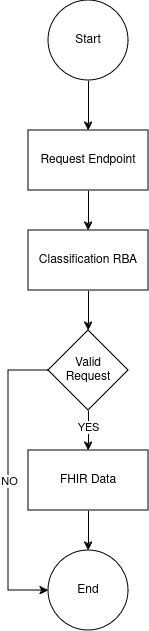
\includegraphics[width=0.2\textwidth]{BAB_TESIS/IMAGES/fhir_rba.drawio.png}
    \caption{Rancangan Integrasi Dengan Sistem FHIR}
    \label{fig:integrasi}
\end{figure}

Gambar \ref{fig:integrasi} dijelaskan proses penggunaan model prediksi Random Forest dengan API, dan bagaimana permintaan data FHIR (Fast Healthcare Interoperability Resources) diproses. Proses dimulai dengan menerima permintaan (Request Endpoint) dari pengguna untuk memperoleh prediksi. Setelah menerima permintaan, sistem kemudian melakukan klasifikasi RBA (Risk-Based Authentication), sebuah langkah untuk mengidentifikasi dan mengevaluasi risiko terkait permintaan tersebut.

Pada tahap berikutnya, sistem mengevaluasi validitas permintaan melalui titik keputusan (Valid Request). Jika permintaan tersebut valid, maka data FHIR yang diminta akan dikirimkan (FHIR Data) dan proses berakhir. Namun, jika permintaannya tidak valid, proses dihentikan tanpa mengakses data FHIR.

Dalam konteks ini, API schema berikut menjelaskan struktur yaml yang digunakan untuk melakukan permintaan prediksi menggunakan model Random Forest:

\begin{lstlisting}
    tags:
      - Prediction
    parameters:
      - name: body
        in: body
        required: true
        schema:
          type: object
          required:
            - features
            - patient_id
          properties:
            features:
              type: array
              items:
                type: number
              example: [5.1, 3.5, 1.4, 0.2]
            patient_id:
              type: string
              example: "example_patient_id"
    responses:
      200:
        description: Prediction result
        schema:
          type: object
          properties:
            prediction:
              type: integer
              example: 1
            observation:
              type: object
      400:
        description: Bad Request
        schema:
          type: object
          properties:
            error:
              type: string
              example: Missing features key in the JSON data
      500:
        description: Internal Server Error
        schema:
          type: object
          properties:
            error:
              type: string
              example: Internal error message
    \end{lstlisting}

    Schema yaml tersebut digunakan dalam permintaan untuk prediksi dengan Random Forest Model. Permintaan ini harus menyertakan dua parameter penting: \texttt{features} dan \texttt{patient\_id}. Parameter \texttt{features} adalah array berisi nilai numerik yang akan digunakan model untuk prediksi, sementara \texttt{patient\_id} adalah string pengidentifikasi pasien yang bersangkutan. Respon yang diberikan oleh API memiliki format JSON yang mencakup hasil prediksi (\texttt{prediction}) dan observasi tambahan (\texttt{observation}), atau deskripsi kesalahan jika terjadi kesalahan saat pemrosesan.

    Secara keseluruhan, diagram dan schema ini menjelaskan alur proses yang harus diikuti untuk melakukan prediksi menggunakan Random Forest Model dan mengakses data FHIR, yang diawali dari penerimaan permintaan hingga penyediaan hasil atau tanggapan kesalahan. Pendekatan ini memastikan adanya langkah-langkah yang terstruktur dan aman dalam pengelolaan serta pemanfaatan data.
    